\documentclass[titlepage,a4paper]{article}

\usepackage{a4wide}
\usepackage[colorlinks=true,linkcolor=black,urlcolor=blue,bookmarksopen=true]{hyperref}
\usepackage{bookmark}
\usepackage{fancyhdr}
\usepackage[spanish]{babel}
\usepackage[utf8]{inputenc}
\usepackage[T1]{fontenc}
\usepackage{graphicx}
\usepackage{float}

\pagestyle{fancy} % Encabezado y pie de página
\fancyhf{}
\fancyhead[L]{TP1S - Max Mustermann}
\fancyhead[R]{Algoritmos y Programación III - FIUBA}
\renewcommand{\headrulewidth}{0.4pt}
\fancyfoot[C]{\thepage}
\renewcommand{\footrulewidth}{0.4pt}

\begin{document}
\begin{titlepage} % Carátula
	\hfill
\includegraphics[width=6cm]{logofiuba.jpg}
    \centering
    \vfill
    \Huge \textbf{Trabajo Práctico 2 — Java}
    \vskip2cm
    \Large [7507/9502] Algoritmos y Programación III\\
    Curso 1 \\ % Curso 1 para el de la tarde y 2 para el de la noche
    Primer cuatrimestre de 2020
    \vfill
    \begin{tabular}{ | l | l | } % Datos del alumno
      \hline
      Alumno: & MUSTERMANN, Max \\ \hline
      Número de padrón: & 123456 \\ \hline
      Email: & mmustermann@fi.uba.ar \\ \hline
  	\end{tabular}
    \vfill
    \vfill
\end{titlepage}

\tableofcontents % Índice general
\newpage

\section{Introducción}\label{sec:intro}
El presente informe reune la documentación de la solución del segundo trabajo práctico de la materia Algoritmos y Programación III que consiste desarollar un juego de quiz que se asimila al Kahoot utilizando las tecnicas de Java, TDD y Git para lograr un trabajo grupal.

\section{Supuestos}\label{sec:supuestos}
% Deberá contener explicaciones de cada uno de los supuestos que el alumno haya tenido que adoptar a partir de situaciones que no estén contempladas en la especificación.

\section{Modelo de dominio}\label{sec:modelo}
% Explicación concisa del diseño general del trabajo.

\section{Diagramas de clase}\label{sec:diagramasdeclase}
% Uno o varios diagramas de clases mostrando las relaciones estáticas entre las clases.  Puede agregarse todo el texto necesario para aclarar y explicar su diseño. Recuerden que la idea de todo el documento es que quede documentado y entendible cómo está implementada la solución.

Kahoot es la clase encargada de empezar el juego y guardar el panel que muestra el juego, las preguntas que se mostraran con sus respectivas respuestas y puntos por responder bien, y sus jugadores con sus respectivos nombres, puntaje y modificadores de puntajes.

\begin{figure}[H]
\centering
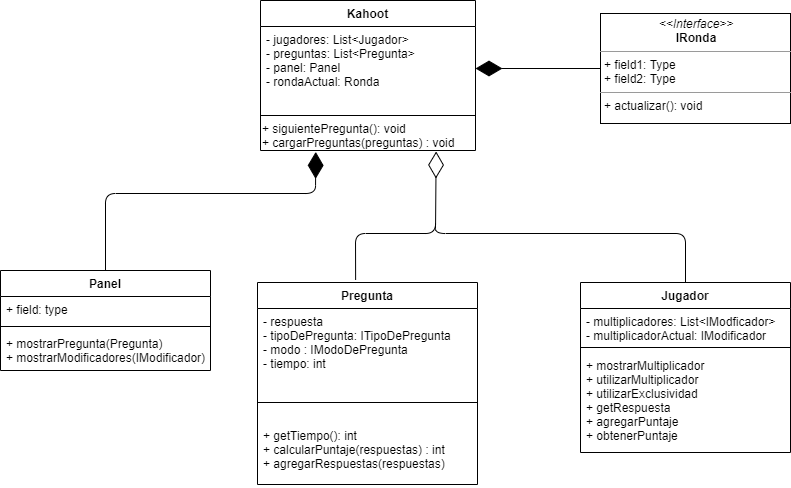
\includegraphics[width=0.8\textwidth]{diagramaGeneral.png}
\caption{\label{fig:class01}Diagrama del Kahoot.}
\end{figure}

\begin{figure}[H]
    \centering
    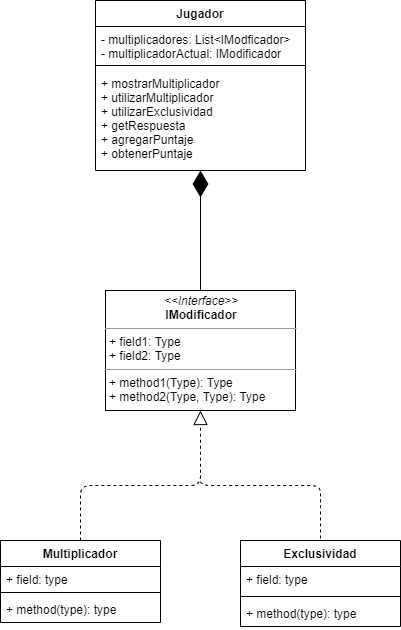
\includegraphics[width=0.8\textwidth]{diagramaJugador.png}
    \caption{\label{fig:class02}Diagrama del Jugador.}
\end{figure}

\begin{figure}[H]
    \centering
    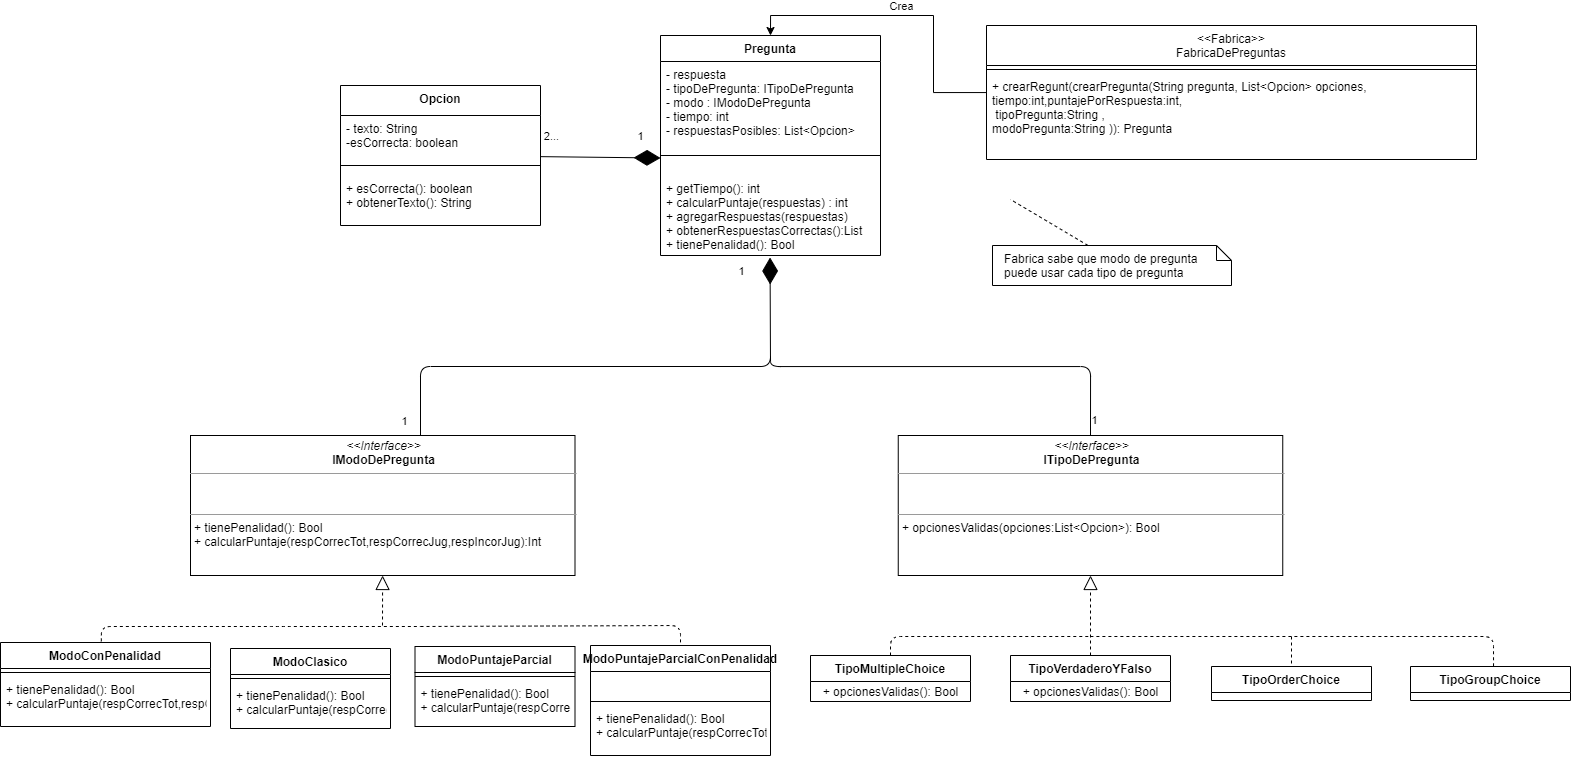
\includegraphics[width=0.8\textwidth]{diagramaPregunta.png}
    \caption{\label{fig:class03}Diagrama de Pregunta.}
\end{figure}

\begin{figure}[H]
    \centering
    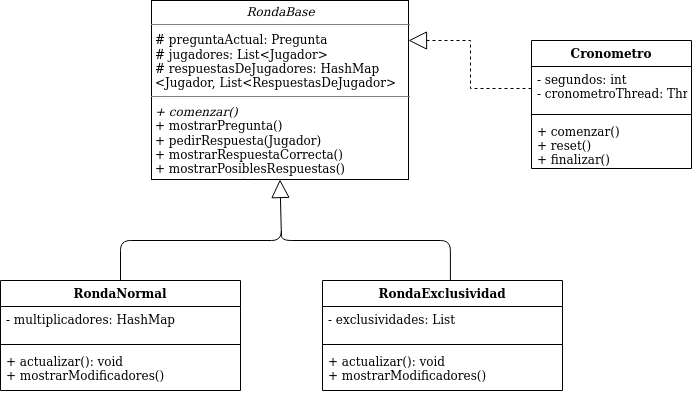
\includegraphics[width=0.8\textwidth]{diagramaRonda.png}
    \caption{\label{fig:class04}Diagrama de Ronda.}
\end{figure}


\section{Detalles de implementación}\label{sec:implementacion}
% Explicaciones sobre la implementación interna de algunas clases que consideren que puedan llegar a resultar interesantes.

\subsection{Aliquam vel eros id magna vestibulum rhoncus}
Sed lorem diam, imperdiet in suscipit sed, lacinia id est. Duis ac turpis at velit tristique dictum ac in augue. Etiam porttitor purus sed nunc scelerisque aliquam. In hac habitasse platea dictumst. Mauris non mauris id lorem iaculis elementum eget quis mi. Aliquam scelerisque porta arcu sed tempus. Duis eleifend euismod laoreet. Aliquam mattis lectus et massa placerat feugiat. Nam mi nisl, rhoncus vel nibh vitae, ullamcorper blandit nibh. Curabitur purus lorem, sollicitudin ut erat eu, pharetra condimentum ante. Nullam imperdiet et neque et tempus. Sed sollicitudin velit molestie pretium iaculis. Praesent eu tincidunt erat. Nulla non fringilla nisi, vel hendrerit felis. Maecenas eget tempor neque.

\begin{verbatim}
| rango |
rango := (2 to: 20) asOrderedCollection.
Transcript show: rango ; cr.
rango copy do: [ :unNumero | unNumero isPrime ifFalse: [ rango remove: unNumero ] ].
Transcript show: rango.
\end{verbatim}

\subsection{Proin sodales leo dapibus sapien fermentum}
Quisque tempus, tortor et convallis interdum, ipsum leo tempus ipsum, in molestie tortor arcu sit amet tellus. Praesent fermentum hendrerit nulla. In maximus ornare maximus. Nullam consectetur placerat enim sit amet lacinia. Etiam pellentesque tellus consectetur hendrerit iaculis. Sed non laoreet felis.

\section{Excepciones}\label{sec:excepciones}
% Explicación de cada una de las excepciones creadas y con qué fin fueron creadas.

\begin{description}
\item[Exception] Lorem ipsum dolor sit amet, consectetur adipiscing elit. Proin nec facilisis odio. Pellentesque habitant morbi tristique senectus et netus et malesuada fames ac turpis egestas. In aliquam dapibus lacus at condimentum. Curabitur ornare scelerisque euismod. Duis a mi in nulla sodales sollicitudin vehicula sit amet sapien. Quisque vel eros ut libero consequat scelerisque. Nullam efficitur ante eu massa gravida sollicitudin.
\item[Excepcion] Curabitur elementum laoreet molestie. Ut hendrerit, quam lobortis porttitor cursus, ex sem facilisis massa, in interdum odio risus hendrerit dui.
\item[Excepcion] Integer porta efficitur felis. Etiam facilisis consectetur sem, ac efficitur orci. Nam a ante commodo, fringilla nisl a, sollicitudin est.
\item[Excepcion] Aliquam erat volutpat. Fusce quis efficitur augue. Fusce egestas mauris a nisi finibus volutpat. Maecenas venenatis ligula ut nisi maximus, vel ultricies enim scelerisque.
\item[Excepcion] Mauris gatis feugiat erat non euismod. Donec sagittis orci enim, et convallis lacus sodales at. Nunc laoreet leo vel metus eleifend, vel aliquam sem tincidunt. Nunc imperdiet eget erat eget tincidunt. Morbi tempus risus quis nulla faucibus facilisis. Sed varius nunc vel neque rutrum vestibulum.
\end{description}

\section{Diagramas de secuencia}\label{sec:diagramasdesecuencia}
% Mostrar las secuencias interesantes que hayan implementado. Pueden agregar texto para explicar si algo no queda claro.

\begin{figure}[H]
\centering
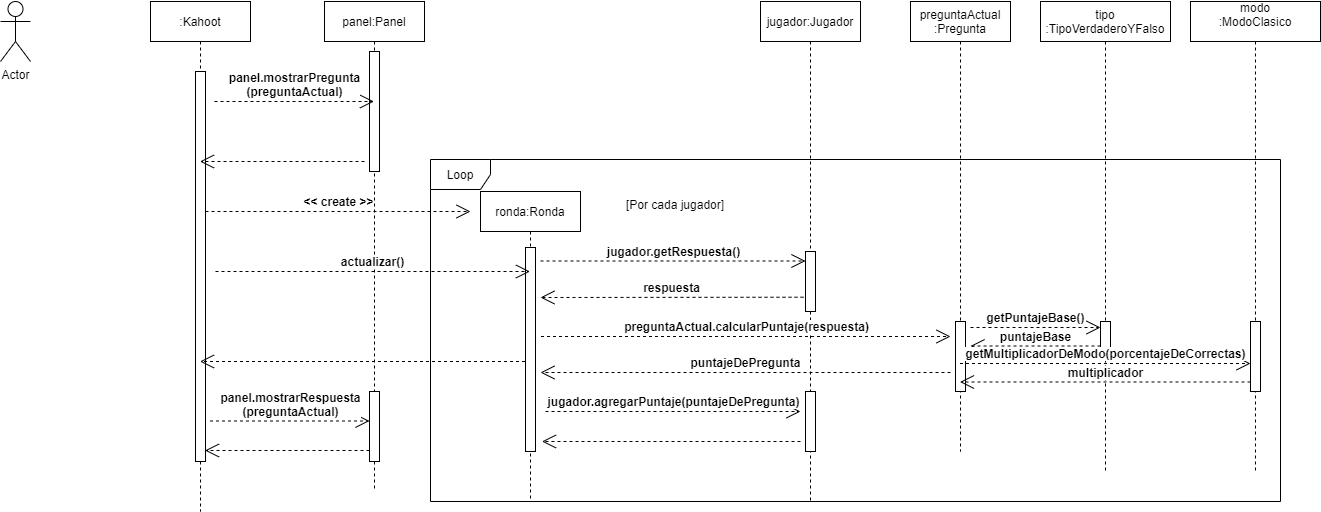
\includegraphics[width=0.8\textwidth]{diagramaDeSecuencia.png}
\caption{\label{fig:seq01}Se muestra el proceso de una ronda en el que un jugador responde una pregunta, se calcula el puntaje y se le agregan los puntos obtenidos.}
\end{figure}


\end{document}
